\documentclass[12pt]{report}

\usepackage{amsmath,amssymb,amsfonts,amsthm}
\usepackage{graphicx}
\usepackage{psfrag}
\usepackage{srcltx}
\usepackage[T2A]{fontenc}
\usepackage[utf8]{inputenc}
\usepackage[english]{babel}
\usepackage{fancyhdr}

\fancypagestyle{plain}{}
\pagestyle{fancy}
\fancyhead{}
\fancyfoot{}
\renewcommand{\headrulewidth}{0 pt}
\rhead{\thepage}
\setlength{\headwidth}{483 pt}
\setlength{\headheight}{0.8 pt}

\paperheight 297mm \paperwidth 220mm \oddsidemargin -7mm
\topmargin 0mm \textwidth 170mm \textheight 220mm \marginparsep
0mm \marginparwidth 0mm \headheight 0mm \headsep 0mm \footskip 5mm
\parskip 2pt

\DeclareMathOperator{\Bool}{Bool}
\newcommand{\Wr}{\mathop{\font\xx=cmsy10 at 18pt \hbox{\xx \char111}}}
\def\thnumbering{chapter}
\def\equa{\Leftrightarrow}
\def\x{{\mathcal{X}}}
\def\b{{\mathcal{B}}}

\newcommand{\bb}[1]{{\bf #1}}
\newcommand{\wsp}{\hspace{6pt}}
\newcommand{\re}{\mathbb{R}}
\newcommand{\nat}{\mathbb{N}}
\newcommand{\Loss}{\mathcal{L}}

\newtheorem{theorem}{Theorem}[section]
\newtheorem{definition}{Definition}[section]

\makeatletter
\renewcommand{\subsection}{\@startsection{subsection}{2}{0mm}{-\baselineskip}{-5pt}{\bf}}
\makeatother


\begin{document}


\renewcommand{\bibname}{References}
\setcounter{tocdepth}{1}

\setcounter{page}{2}

\large

\thispagestyle{empty}
\tableofcontents


\chapter*{Introduction}
\addcontentsline{toc}{chapter}{Introduction}

The problem of text spam has been around since the early days of e-mail services and has since evolved to numerous forms. Spam can vary by platform (e-mail, instant messaging, social network messaging), by intentions (from advertisement to phishing and ransom), by distribution targets (from a single individual or general public), etc.

While the number of messaging domains is growing rapidly, the prime purpose of spam remains the same: to reach out to the recipient by any means or to trick him into acting on the message by disguising it as a legitimate message. This leads to a very clear practical definition of spam from user's perspective as \textit{any unsolicited message}, whether it acknowledges its origin (e.g. unwanted advertisement) or is crafted to gain the user's trust (e.g. targeted phishing and ransom attacks).

Given the large number of messaging systems to which spam is applicable, the problem of detection of unwanted correspondence has evolved along with distribution methods and now includes additional metadata like attached media and hyperlinks. While they may seem to increase the complexity of spam detection, they in fact give a basis for additional means of filtering which are often much easier to perform than the raw text classification.

While the message metadata can provide additional information, in practice text classification is inevitable. It is usually the final step in the whole process as it tends to be most computationally expensive. Since the metadata processing is different from case to case, it is safe to say that the general problem of spam filtering comes down to binary text classification. Therefore, it makes sense to develop universal methods for spam classification of text messages that can be later adopted to any domain.

A number of supervised machine learning techniques have been successfully applied to spam filtering. They, however, have not yet fully replaced regular expression based filtering in large scale commercial applications due to high requirements and sensitivity to false positives.

In this thesis we give an overview of a number of statistical methods of performing spam filtering on text messages, including Bayesian classifiers, nearest neighbors, neural networks and SVM. The mainly focus on the high level algorithm and provide space and time complexity limits for each of the algorithms.

The main focus of this work is the Bayesian classifier - one of the most common and effective approaches to spam filtering. We analyze an existing naive Bayesian approach and tackle some of the false assumptions that the algorithm relies on. We then give performance comparison between the resulting algorithm to the original classifier.

Additionally, we give an brief overview of common problems in text message classification like feature selection. Finally, we provide a performance comparison of detailed algorithms in practice.

\newpage


\chapter{Statement of the Problem}

\section{Scope and Applications}

The vast majority of massively used communication services rely on text messages as the main form of information exchange. Because of their openness, such networks be extremely useful in spreading malicious messages across wide audiences, both via private (addressed to a particular individual) and public messages. Conceptually social network spam is no different from e-mail spam as private messaging services of popular social networks are equivalent in their functionality to e-mail. Hence, we can focus the problem of classifying spam messages in general, regardless of the platform.

In general, the problem of spam detection depends heavily on the application's domain and can benefit from additional metadata available along with the text message. For example, in case of e-mails the mail header is the source of metadata. Modern spam filtering systems detect the vast majority of malicious mails by simply checking the sender's reputation before proceeding with analysis of the message body.

This, of course, applies to all messaging services. Maximum effectiveness can not be achieved without using all available data in addition to the message text. However, in most cases text analysis is the second stage preceded by a domain-specific filter. Therefore, we can further focus on statistical classification of spam for text messages without specific constraints.

The entities we need to classify are text messages that are given in the form of strings. Raw strings are not convenient objects to handle in this case since most machine learning algorithms can only classify numerical objects or require a distance metric or other measure of similarity between the objects.

Before proceeding with machine learning we have to convert all messages to numerical vectors called \textit{feature vectors}, and then classify these vectors. The simplest example of a feature vector is a binary vector each index of which specifies whether a certain word is present in the message or not. More complex feature vectors may contain frequencies of words.

Extraction of features usually means that some information from the original message is lost. On the other hand, the way feature vector is chosen is crucial for the performance of the filter. However, feature vectors have to be sensitive to the class of the message. If the features are chosen so that there may exist a spam and a legitimate message with the same feature vector, any algorithm will make mistakes on it.

Preserving information with feature vectors is not trivial and usually means that some information is lost. Even the ultimate feature vector containing frequencies of \textit{all} words in the message does not preserve semantical information. This problem however is out of scope and is in the domain of Natural Language Processing. In most practical applications the most basic vectors of word frequencies or its modification are sufficient.

Note that at the stage of feature selection it is possible to include the features from the available metadata along with features from message text. However, we will only focus on plain text as any of the described algorithms can be easily expanded.

\newpage

\section{Definitions and Notations}

Let us give a number of definitions that will be commonly used.

$M$ - the set of all messages.

$L \subseteq M$ - the set of legitimate messages.

$S = M \setminus L$ - the set of spam messages.

Note that we will often speak of $M$, $L$ and $S$ in context of the set of training messages.

$T = \{(m_1, c_1), (m_2, c_2), ..., (m_k, c_k)\}, m_i \in M, c_i \in \{S, L\}, 1 \leq i \leq k$ - the training set of already classified messages.

$T_c = T \cap c, c \in \{L, S\}$ - training set of legitimate ($T_L$) or spam ($T_S$) messages.

$x = (x_1, x_2, \dots, x_n), x_i \in \{0, 1\}, 1 \leq i \leq n$ - binary feature vector of a message. Each coordinate specifies whether a specific feature applies to the message (i.e. whether the corresponding word is present in the message).

$f : M \rightarrow \{S, L\}$ - classification function that given a message determines its class. This function is the ultimate goal of any classification algorithm.

We will also use the following symbols with fixed meanings:

$n$ - the number of features used in classification.

$k = |T|$ - the power of the training set.

\newpage


\chapter{Basic Methods}

\section{Naive Bayes Classifier}

Consider the simple case of text classification based on the presence or absence of just one word $W$. Suppose we know that the word $W$ only occurs is spam messages. This gives us confidence that any message containing $W$ is spam. This approach can be generalized to the probability of a message feature vector occurring in the message.

Suppose we have two classes $L$ and $S$ corresponding to legitimate and spam messages, and that there is a known probability distribution of feature vectors $P(x | c), c \in \{L, S\}$. In general it is hard to define such distribution, but it is often possible to provide an approximation. What we need to obtain is the class that the given message belongs to, or the probability $P(c | x)$. This can be done using the Bayes' formula

$$P(c | x) = \dfrac{P(x | c) P(c)}{P(x)} = \dfrac{P(x | c) P(c)}{P(x | L) P(L) + P(x | S) P(S)}$$

where $P(x)$ is the a-priori probability of a message with feature vector $x$ and $P(c)$ is the probability of class $c$, i.e. the probability that any given message belongs to $c$. Given the values $P(c)$ and $P(x | c)$ for $c \in \{L, S\}$ one can calculate the probability $P(c | x)$ which can then be used in a classification rule.

The most basic classification rule is to classify message to the category with bigger probability.

\begin{definition}
	Maximum a-posteriori probability (MAP) rule: if $P(S | x) > P(L | x)$ then classify $x$ as spam, otherwise classify as legitimate message.
\end{definition}

The MAP rule can be transformed to

\begin{center}
	If $\dfrac{P(x | S)}{P(x | L)} > \dfrac{P(L)}{P(S)}$ then classify $x$ as spam, otherwise as legitimate message.
\end{center}

The ratio $\dfrac{P(x | S)}{P(x | L)}$ is known as the \textit{likelihood ratio} and is denoted as $\Lambda(x)$.

This approach can be too simplistic for certain applications. For example, in case of e-mail spam filtering, false positives (classifying legitimate message as spam) are usually much more unwanted than false negatives (classifying spam as legitimate message). The following generalization allows to take such restrictions into account.

\begin{definition}
	A cost function $\Loss(c_1, c_2)$ denotes the cost of misclassifying a message of class $c_1$ as the one belonging to class $c_2$.
\end{definition}

Then we can express the expected risk of classifying a message $x$ belonging to class $c$ in the above terms.

\begin{definition}
	The function $R(c | x) = \Loss(S, c) P(S |x) + \Loss(L, c) P(L | x), x \in M, c \in \{L, S\}$ is called the risk function.
\end{definition}

Now we can define a natural classification rule in terms of expected risk.

\begin{definition}
	Bayes' classification rule: if $R(S | x) < R(L | x)$ then classify $x$ as spam, otherwise as legitimate message \cite{Kecman}.
\end{definition}

It can be shown that Bayesian classifier $f$ minimizes the average risk

$$R(f) = \int \Loss(c, f(x)) dP(c, x) = P(L) \int \Loss(L, f(x))dP(x | L) + P(S) \int \Loss(S, f(x))dP(x | S)$$

so in this sense Bayesian classifier already is optimal \cite{Tretyakov}.

Naturally, the loss of classifying the message correctly is zero, thus $\Loss(S, S) = \Loss(L, L) = 0$. Then the Bayes's classification rule can be rewritten as

\begin{center}
	If $\Lambda(x) > \lambda \dfrac{P(L)}{P(S)}$ classify as spam otherwise as legitimate message.
\end{center}

Here $\lambda = \dfrac{\Loss(L, S)}{\Loss(S, L)}$ is the additional parameter that specifies the risk of misclassifying legitimate messages as spam. As the value of $\lambda$ increases, the classifier produces fewer false positives. This makes Bayesian classifier especially appealing in e-mail spam filtering since false positives there are much more expensive than false negatives.

While the classification process is straightforward, the practical applications of Bayes's classifier are limited by our ability to approximate the a-priori probabilities $P(x | c)$ and $P(c), c \in \{L, S\}$ from the training data. Therefore, while the Bayes's classifier is optimal in the sense of minimizing the loss of classification for given a-priori probabilities, the quality of spam detection depends on the feature selection and approximation of these probabilities.

$P(L)$ and $P(S)$ can be easily approximated by the ratio of legitimate and spam messages respectively. $P(x | c)$, however, is non-trivial and depends on the contents of selected feature vector.

Consider the simplest case where the feature vector $x_w$ is $1$ if the message contains $w$ and $0$ otherwise. Then the probability $P(x_w = 1 | S)$ can be approximated by the ratio of spam messages containing $w$ to the ratio of all spam messages in a training set. This is sufficient to be used by the Bayes's classifier, so we can outline the training and selection process for this model.

\textbf{Training process}

\begin{enumerate}
	\item Calculate probabilities $P(c)$, $P(x_w = 0 | c), P(x_w = 1 | c), c \in \{L, S\}$.
	\item Using Bayes's formula calculate $P(c | x_w = 0)$ and $P(c | x_w = 1)$.
	\item Calculate $\Lambda(x_w), x_w = 0, 1$, calculate $\lambda \dfrac{P(L)}{P(S)}$ and store these values.
\end{enumerate}

\textbf{Classification process}

\begin{enumerate}
	\item Determine feature vector $x_w$ for message $m$.
	\item Retrieve the stored value $\Lambda(x_w)$.
	\item Use Bayes's decision rule to determine class of the message.
\end{enumerate}

Now we need to generalize this classifier to include more features than just the presence of a single word. The simplest way (and the most used one) is to choose a subset of words $w_1, w_2, \dots, w_n$ and define the feature vector $x = (x_1, x_2, \dots, x_n)$, $x_i = 1$ if the message contains $w_i$, and $x_i = 0$ otherwise.

The problem with this approach is that it requires calculation and storing of all possible values of the feature vector, which is not feasible since there are $2^n$ such vectors. A common way to remove this requirement is to assume that the individual components of the vector are independent \cite{Zhang}. This assumption is not formally correct, but in practice it is a good compromise between formal correctness and computational requirements. We will consider other options in later chapters.

Because of independence of features:

$$P(x | c) = \prod_{i=1}^{n}P(x_i | c)$$
$$\Lambda(x) = \prod_{i=1}^{n}\Lambda_i(x_i)$$

This classifier is known as Naive Bayesian Classifier due to assumption of independence of features. Training and classification are very simple computationally.

\textbf{Training process}

\begin{enumerate}
	\item For all $w_i \in W$ calculate and store $\Lambda_i(x_i), x = 0, 1$.
	\item Calculate and store $\lambda \dfrac{P(L)}{P(S)}$.
\end{enumerate}

\textbf{Classification process}

\begin{enumerate}
	\item Determine feature vector $x$ for message $m$.
	\item Calculate $\Lambda(x)$ using the stored values $\Lambda_i(x_i)$.
	\item Use Naive Bayes's decision rule to determine class of the message.
\end{enumerate}

In terms of word selection for the feature vector, usually most common and most rare words are excluded. For simple cases when performance is not critical, all words form the training set can be used. In later chapters we will consider ways to select words with maximum mutual information.

Another benefit of naive Bayesian filter is that it is very easy to expand the feature vector to include additional available metadata. In case of e-mails, for example, it would be contents of e-mail headers. It is possible to include additional components either to the calculation of the a-priory probability of the vector or to combine the risk of Bayesian classifier with additional risk calculated from metadata when making a decision.

\newpage

\section{k Nearest Neighbors Classifier}

$k$ Nearest Neighbors (or $k$-NN) is a modification of the classical Nearest Neighbors algorithm. The idea behind this classifier is to first define a metric on feature vectors and then classify the message according to classes of $k$ nearest messages in the training set. The metric is often chosen to be Euclidean, but Hamming or $l_p$ can also be used for this purpose.

\textbf{Training process}

\begin{enumerate}
	\item Store feature vectors of training messages in two sets $L$ and $S$.
\end{enumerate}

\textbf{Classification process}

\begin{enumerate}
	\item For message with feature vector $x$ determine $k$ nearest neighbors from messages in the training set. If there are more legitimate messages among them, classify $x$ as legitimate message, otherwise classify as spam.
\end{enumerate}

Since the algorithm does not require any preprocessing of the training dataset, the training process is trivial. The classification process, however, requires calculation of distances to all messages in the training set, and for feature vectors of length $m$ the most trivial implementations take $O(mn)$ time for set of $n$ messages in case of Hamming or $l_p$ metrics. Performing indexing on the training set can decrease the running closer to $O(n)$ \cite{Tretyakov}. However, if the size of the set increases over time, the algorithm might not be feasible in practice for certain applications.

The $k$-NN classifier is widely applicable in general classification problems, partially because it is one of so called \textit{universally consistent} rules. Consider the training set $s_n$ of $n$ samples, and let use denote the $k$-NN classifier over that set as $f_{s_n}$. Similar to Bayesian classifier, we can determine the average risk $R(f_{s_n})$ of the classifier. The risk value is always greater than or equal than the Bayesian risk $R_*$ (recall that Bayesian classifier is optimal in this sense), however for large values of $n$ $R(f_{s_n})$ will be close to $R_*$.

\begin{definition}
	A classification rule is called consistent if the expectation of the average risk $E(R_n)$ converges to the optimal (Bayesian) risk $R_*$ as $n$ goes to infinity:
	$$E(R_n) \xrightarrow[n \rightarrow \infty]{} R_*$$.
	The classification rule is called universally consistent if it is consistent for any distribution of $(x, c)$.
\end{definition}

\begin{theorem}[Stone, 1977]
	If $k \rightarrow \infty$ and $\frac{k}{n} \rightarrow 0$, then $k$-NN classification rule is universally consistent.
\end{theorem}

Consistency of $k$-NN rule allows to increase the quality by increasing the size of the training set. Stone theorem guarantees that as the size of the training set increases with constant value of $k$, the selection of messages for the training set does not matter. In addition to this, small values of $k$ prevent quadratic complexity $O(n^2)$ when computing nearest neighbors.

Despite theoretical results, $k$-NN classifiers are performing worse than competition in practice for spam classification and are computationally expensive.

\newpage

\section{Artificial Neural Network Classifier}

Artificial neural networks (ANN) is a family of models inspired by biological neural networks which are widely used in classification, regression and density estimation by approximating functions that can depend on a large number of inputs and are generally unknown. A neural network is a complex function that may be decomposed into smaller units called neurons and represented graphically as a network. Many functions fall under such criteria, however the most common kinds of neurons are perceptron and multilayer perceptron.

The perceptron produces a linear function of the feature vector $f(x) = w^Tx + b$ where $f(x) > 0$ for vectors of one class and $f(x) < 0$ for vectors of another class. Here $w$ is the vector of weights, or \textit{bias}, $w = (w_1, w_2, \dots, w_n)$. This vector will be determined by the training process.

If we denote the classes by number -1 and +1, we can use $d(x) = sign(w^Tx + b)$ as decision function. This allows us to represent the decision function graphically as a neuron with $n$ inputs and a single output. A system of one perceptron is an example of the simplest neural network.

Suppose the feature vector is two-dimensional, $x \in \re^2$. Then we can represent these feature vectors as points on the plane. Then the decision function can be represented as a line dividing the plane in two parts, each corresponding to one of the classes. Similarly, the decision boundary for three-dimensional feature vectors is a plane, etc. In general, for $n$-dimensional feature vector the decision boundary is a $n$ - dimensional hyperplane.

The learning process for a perceptron is iterative. The initial values of parameters $(w_0, b_0)$ can be arbitrary, as they are updated on each iteration. On the $k$-th iteration of the algorithm a training sample $(x, c)$ is chosen such that the current decision function does not classify it correctly, i.e. $sign(w_k^Tx + b_k) \ne c$. Then the parameters $(w_k, b_k)$ are then updated according to the rule:

$$w_{k+1} = w_k + cx$$
$$b_{k+1} = b_k + c$$

The algorithm terminates when a decision function that correctly classifies all training set is found. If the training set is linearly separable, the perceptron algorithm converges. It is known as Perceptron Convergence Theorem proven by Frank Rosenblatt in 1962 \cite{Cristianini}. If, however, the set is not linearly separable, the algorithm will never converge. In this case it is possible to still use the perceptron, but the training loop needs to stop when the number of misclassification becomes small.

We can now outline the training and classification phases of the perceptron.

\textbf{Training process}

\begin{enumerate}
	\item Initialize the values of $w$ and $b$ with random values or 0.
	\item Find a sample from the training set $(x, c)$ such that $sign(w^Tx + b) \ne c$. If there are no such samples, terminate as the training is completed and all training samples are being classified correctly, else proceed to the next step.
	\item Update $(w, b)$ with new values $w := w + cx$, $b := b + c$ and go to the previous step.
\end{enumerate}

\textbf{Classification process}

\begin{enumerate}
	\item For message with feature vector $x$ classify it as $sign(w^Tx + b)$.
\end{enumerate}

As mentioned before, perceptrons can be combined in multiple layers to form \textit{multilayer perceptrons} which are non-linear classifiers. Neurons of the first layer which takes in the input parameters are called \textit{input neurons}, similarly neutrons of the last layer which provide the function result value are called \textit{output neurons}. All layers between input and output are called \textit{hidden layers}.

Each neuron in the networks is similar to a perceptron: for input vector $x = (x_1, x_2, \dots, x_n)$ it calculates output value by the formula

$$o = \phi(\sum_{i = 1}^{n}w_i x_i + b)$$

where $w_i$ and $b$ are weights and bias of the neuron respectively, $\phi$ is a nonlinear function that approximates binary output of the perceptron. Most often $\frac{1}{1 + e^{ax}}$ or $\tanh(x)$ are used as $\phi$ as they tend to give a good approximation while being mathematically convenient.

Like in the case of a single perceptron, training of a neural network is searching for the values of weights and biases for all neurons that minimize the output error. Let us denote $f(x)$ as the output of the neural network. Then for training samples $(x_i, c_i), 1 \leq i \leq k$ the training has to minimize the \textit{total training error}

$$E(f) = \sum_{i = 1}^{k}|f(x_i) - c_i|^2$$

An iterative algorithm can be used to perform this minimization. The most common one is the gradient descent which in case of neural networks is called \textit{error backpropagation}. The theory of backwards propagation of errors is well developed and has many implementations in practice \cite{Haykin}.

The main reason to use multiple layers of neurons is that the multilayer neural network is a non-linear classifier. As a result, they are applicable for tasks with training data that is not linearly separable, particularly when the number of features is relatively small. However, in case of spam detection with multiple words being used as features the data is often linearly separable, thus using neural network will have no noticeable benefits over a simple perceptron.

Performance of the neural network is proportional to the number of neurons. Thus, the large number of features directly impacts performance as it translates to increased number of input neurons and thus the complexity of the network in total. In practice the number of features would have to be more strictly limited than in case of a perceptron, which for spam detection means the trade-off between non-linear decision boundaries and the amount of information loss.

Because of the above reasons and due to the large number of parameters that require tuning. the multilayer perceptron is hard to use in practice for spam detection. It has been successfully used for that purpose \cite{Tretyakov}, but it is not easily applicable in general case as it is hard to reconfigure. For the purposes of this thesis we shall focus on a simple perceptron.

\newpage

\section{SVM Classifier}

Support Vector Machines (SVM) is a class of widely used algorithms for classification and regression. The theoretical foundation of SVM is the Statistical Learning Theory that gives certain guarantees of performance \cite{Cristianini}. Let us consider classification problem with SVM for linearly separable data.

SVM works in a similar manner to perceptron in terms of finding a linear boundary that separates test data according to their classes. However, the purpose of SVM is not to find any of these boundaries if they exist, but to find the maximal margin separating hyperplane, with maximum distance to the nearest training sample.

\begin{definition}
	Let $X = \{(x_i, c_i)\}$, $x_i \in \re^n$, $c_i \in \{-1, +1\}$ be the set of training samples and $(w, b)$ denote a separating hyperplane $sign(w^T x_i + b) = c_i$ for all $1 \leq i \leq k$. The margin $m_i$ of a training sample $(x_i, c_i)$ with respect to the separating hyperplane is the distance from $x_i$ to the hyperplane
	
	$$m_i = \dfrac{|w^T x_i + b|}{||w||}$$
	
	The margin $m$ of the separating hyperplane for training set $X$ is the smallest margin of an instance in the training set
	
	$$m = \min_i m_i$$
	
	The maximal margin separating hyperplane for training set $X$ is the separating hyperplane with maximal margin with respect to the training set \cite{Tretyakov}.
\end{definition}

The hyperplane given by parameters $(x, b)$ is the same as the hyperplane given by parameters $(kx, kb)$, hence we can only consider hyperplanes for which $\min_i |w^T x_i + b| = 1$. The optimal canonical hyperplane has minimal value of $||w||$, and that in order to find a canonical hyperplane we need to solve the minimization problem: minimize $\frac{1}{2} w^T w$ given conditions

$$c_i(w^T x_i + b) \ge 1, i = 1, 2, \dots, k$$

The problem may be transformed to a certain dual form: maximize

$$L_d(\alpha) = \sum_{i = 1}^{k} \alpha_i - \frac{1}{2} \sum_{i, j = 1}^{k} \alpha_i \alpha_j c_i c_j x_i^T x_j$$

with respect to dual variables $\alpha = (\alpha_1, \alpha_2, \dots, \alpha_k)$, $\alpha_i \ge 0 \forall i$ and $\sum_{i = 1}^{k} \alpha_i c_i = 0$ \cite{Tretyakov}.

The resulting problem is a classical quadratic optimization problem, for which there exist efficient solutions. Once we have found the solution $\alpha$, parameters $(w_o, b_o)$ of the optimal hyperplane are determined as

$$w_o = \sum_{i = 1}^{k} \alpha_i c_i x_i$$

$$b_o = \frac{1}{c_m} - w_o^T x_k$$

where $m$ is an arbitrary index for which $\alpha_m \ne 0$.

The resulting hyperplane is defined by the training samples that are at minimal distance to it, so called \textit{support vectors}. Training process is quite complex, while classification is straightforward.

\textbf{Training process}

\begin{enumerate}
	\item Find $\alpha$ that solves the dual problem (maximizes $L_d$ under named
	constraints).
	\item Determine $w$ and $b$ for the optimal hyperplane and store the values.
\end{enumerate}

\textbf{Classification process}

\begin{enumerate}
	\item For message with feature vector $x$ classify it as $sign(w^T x + b)$.
\end{enumerate}

Implementation of SVM is non-trivial, in particular because of the quadratic optimization problem. In case of spam classification, an easy and quick classification process is undoubtedly a benefit. However, in many cases of spam filtering the training set needs to be regularly updated, which is a hard procedure with SVM.

\newpage


\chapter{Modified Bayesian Classifier}

\section{Non-Naive Bayesian Classification}

\subsection{Overview}

Recall the naive Bayesian classifier described earlier. Let us ignore feature selection for now and instead only consider classification of feature vectors. Bayesian classifier is optimal in the sense of minimization of expected risk, however it is a common practice to assume that individual components of the feature vector are independent. Such assumption, while significantly simplifying implementation and improving training and classification performance, does compromise the optimality of the classifier. In this chapter we will analyze the possibility of an effective Bayesian classifier without assumption about feature independence and will develop an algorithm that allows to balance learning/classification speed with optimality guarantees.

Let us return to Bayesian model for the case of a single feature.

\textbf{Training process}

\begin{enumerate}
	\item Calculate probabilities $P(c)$, $P(x_w = 0 | c), P(x_w = 1 | c), c \in \{L, S\}$.
	\item Using Bayes's formula calculate $P(c | x_w = 0)$ and $P(c | x_w = 1)$.
	\item Calculate $\Lambda(x_w), x_w = 0, 1$, calculate $\lambda \dfrac{P(L)}{P(S)}$ and store these values.
\end{enumerate}

\textbf{Classification process}

\begin{enumerate}
	\item Determine feature vector $x_w$ for message $m$.
	\item Retrieve the stored value $\Lambda(x_w)$.
	\item Use Bayes's decision rule to determine class of the message.
\end{enumerate}

In the naive version assumption about independence of features was made. With this assumption the required probability can be easily found from a-priori probabilities of separate features:

$$P(x | c) = \prod_{i=1}^{n}P(x_i | c)$$

Now we again need to generalize this classifier to include multiple features, however this time without making any assumptions about the underlying distribution. Let us ignore the feature selection for now as it will be described in the following chapter.

Consider the feature vector $x = (x_1, x_2, \dots, x_n)$, $x_i = 1$ if the message contains $w_i$, $x_i = 0$ otherwise. As mentioned before, calculating and storing this value for all $2^n$ possible combinations of feature vector $x$ is not feasible in practice, so this has to be done during classification process.

The probability $P(x | c)$ for any given $c \in \{L, S\}$ is equal to the ratio of messages in $c$ with feature vector $x$ to all messages in $c$. To calculate it efficiently, we need to be able to quickly determine the number of messages in the set that have specified feature vectors. This can be done in a number of ways.

\subsection{Non-Naive Bayesian Classification Algorithm}

Let us now outline the updated algorithm for training and classification. Let $M(c, x), c \in \{L, S\}, x \in 2^{|n|}$ denote the power of subset of $c$ with feature vector $x$.

\begin{theorem}
	\textbf{Non-naive Bayesian classification algorithm}
	
	\textbf{Training process}
	
	\begin{enumerate}
		\item Calculate $|L|$ and $|S|$. Time complexity: $O(k)$.
		\item Calculate likelihood ratio $\lambda \frac{P(L)}{P(S)}$. Time complexity: $O(1)$.
		\item For both $L$ and $S$ construct corresponding tries that allow to perform lookup of $M(c, x)$. Time complexity: $O(nk)$. Space complexity: $O(nk)$.
	\end{enumerate}
	
	\textbf{Classification process}
	
	\begin{enumerate}
		\item Determine feature vector $x$ for message $m$. Time complexity: $O(|m|)$ where $|m|$ denotes the number of words in message $m$.
		\item Perform lookup of $M(L, x)$ and $M(S, x)$ using the tries. Time complexity: $O(n)$.
		\item Calculate $P(x | L) = \frac{M(L, x)}{|L|}$ and $P(x | S) = \frac{M(S, x)}{|S|}$. Calculate $\Lambda(x) = \frac{P(x | S)}{P(x | L)}$. Time complexity: $O(1)$.
		\item Use Bayes's decision rule to determine class of the message. Time complexity: $O(1)$.
	\end{enumerate}
\end{theorem}

\begin{proof}
	To be able to perform lookup of the number of messages with specific feature vector, we shall store the known feature vectors in a trie where each node corresponds to one of the features, starting from $x_1$. Given a node at position $x_i$ the left subtree will contain vectors with $x_i = 0$ and the right subtree - vectors with $x_i = 1$. The leaf nodes will contain the number of messages in the set with feature vectors that match the path from root to leaf. Since we need to calculate both $P(x | L)$ and $P(x | S)$, we shall maintain two tries, one for legitimate messages and one for spam.
	
	With this representation adding a message to the trie takes time $O(n)$ (where $n$ is the dimension of feature vector) since the length of the path from root to the corresponding leaf node is $n$. Therefore, the whole training process takes $O(nk)$, where $k$ is size of the training set.
	
	Lookup of the feature vector also takes linear time $O(n)$ since we only follow the path of length $n$ from root to a leaf node. It is also easy to show that the lower bound is $O(n)$ because each of the feature vectors has to be examined at least once. Therefore, our algorithm is optimal.
	
	The amount of extra storage required by the trie is $O(nk)$ (consider the set of one message). Obviously, some fractions of the paths will be shared (different messages with identical feature vectors will share the whole path). One way to increase the number of shared nodes is to sort the features in descending order by the number of messages that have the same value of this feature, then more messages will share common beginning of the path.
	
	Of course, this is not the only way to store and perform lookup on feature vectors. We can also use a hash table. Calculating hash of the feature vector is $O(n)$. Construction and lookup are $O(nk)$ and $O(n)$ on average respectively, however they can be $O(n^2k)$ and $O(n^2)$ in the worst case. For our purpose it will be sufficient to focus on trie approach.
\end{proof}

\subsection{Generalizing Probability of Feature Vectors}

In case of naive approach only probabilities of separate features need to be stored. They are sufficient to determine the overall probability of the feature vector for all $2^n$ combinations, regardless of whether they are present in the training set. In the approach described above, however, only the information about concrete feature vectors from the training set is stored. While it is possible to calculate probability of any feature vector in the training set by the algorithm above, in its current version probability of any feature vector that is not in the training set to be in either $L$ or $S$ is $0$. In fact, probability of any message $m$ to belong to $c$ will be non-zero if and only if the training set contains at least one message with identical feature vector.

This can be interpreted as excessive 'formality', i.e. the algorithm produces the optimal result, but in the context of given training set. We would naturally want to get a reasonable approximation of the probability of messages that are not present in the training set. Note that out of $2^n$ possible feature vectors at most $k$ will be present in the constructed trie, and the probability that the algorithm will produce the expected result is $\frac{k}{2^n}$ at best. Therefore, without providing an alternative probability for unrecognized feature vectors these modifications will be useless in practice.

One possible solution is to fall back to naive Bayesian classifier for all feature vectors that are not present in the training set. In this case, our modified classifier will only produce different results for a small fraction of possible messages ($\frac{k}{2^n}$), making these modifications negligible in practice. For example, even if we assume that the training set contains $k_u$ unique feature vectors, for $k_u <= 2^30$, (i.e. the training set is very unlikely to contain more than 1 billion messages in practice) $n$ has to be not larger than $log_2(k) = 30$. Obviously, we want to include significantly more features.

\newpage

\section{Semi-Naive Bayesian Classification}

At this point we have an optimal algorithm for any message such that its feature vector is present in the training set. In this section we will describe a number of ways to give an approximation of conditional probabilities for all possible feature vectors.

\subsection{Chain rule}

We can express probability $P(x | c), c \in \{L, S\}$ in terms of conditional probabilities using the chain rule:

\begin{center}
	$P(x | c) = P(x_1 | c) P(x_2 | x_1, c) P(x_3 | x_1, x_2, c) \dots P(x_n | x_1, x_2, \dots, x_{n - 1}, c) = \prod_{i=1}^{n}P(x_i | \bigcap_{j = 1}^{i - 1} x_j, c)$
\end{center}

Let us first consider any of the probabilities $P(x_i | x_1, x_2, \dots, x_{i-1}, c)$ for given values of $x_1, \dots, x_{i - 1}$ and $c$. The constraint of $c$ limits the set of messages to either only legitimate messages or only spam. The constraints on the fist $i - 1$ features require the first $i - 1$ components of the feature vector to be equal to given values $(x_1, x_2, \dots, x_{n-1})$.

We will now extend the function $M$ from the previous section to be able to compute the number of features with constraints on some indexes. Let $M(c, x_1, x_2, \dots, x_l)$, $1 \leq l \leq n$ denote the power of subset of $c$ with the first $l$ features equal to $x_1, x_2, \dots, x_l$. Then

\begin{center}
	$P(x_i | x_1, x_2, \dots, x_{i-1}, c) = \dfrac{M(c, x_1, x_2, \dots, x_i)}{M(c, x_1, x_2, \dots, x_{i-1})}$
\end{center}

The value of $M(c, x_1, \dots, x|i)$ is the number of messages in the training set of legitimate or spam messages (depending on $c$) feature vectors of which start with $x_1, x_2, \dots, x_i$. One way to find this value is to go through all training messages of category $c$ and count the number of those with feature vectors that match $x_1, \dots, x_n$. This would mean $O(nk)$ time complexity for each probability in the chain, and overall complexity for $P(x | c)$ would be $O(\sum_{i=1}^{n} nk) = O(n^2 k)$, which is, of course, not feasible in practice.

However, we can reuse the trie that we already are using for calculating $M(c, x_1, \dots, x_n)$, only in this case we need to retrieve the number of messages feature vector of which matches the first $i$ given coordinates. This can be done in $O(n)$ if in each node we store the sum of values of all terminal nodes in the subtree rooted at that node. This will give us exactly the number of messages feature vector of which satisfies the constraints on the first $i$ coordinates.

In fact, as we follow the path in the trie, on each step we will calculate exactly one of the probabilities in the chain. Taking their product gives us the final probability with overall complexity of $O(n)$. Essentially, this approach is just a different computation of the same non-Bayesian classifier, but it can be modified more easily.

\subsection{Chain Rule Bayesian Classification Algorithm}

Let us outline the final version of semi-naive Bayesian classifier based on chain rule computation.

\begin{theorem}
	\textbf{Chain rule Bayesian classification algorithm}
	
	\textbf{Training process}
	
	\begin{enumerate}
		\item Calculate $|L|$ and $|S|$. Time complexity: $O(k)$.
		\item Calculate likelihood ratio $\lambda \frac{P(L)}{P(S)}$. Time complexity: $O(1)$.
		\item For both $L$ and $S$ construct corresponding tries that allow to perform lookup of $M(c, x_1, x_2, \dots, x_i), 1 \le i \le n$. Time complexity: $O(nk)$. Space complexity: $O(nk)$.
	\end{enumerate}
	
	Time complexity: $O(nk)$. Space complexity: $O(nk)$.
	
	\textbf{Classification process}
	
	\begin{enumerate}
		\item Determine feature vector $x$ for message $m$. Time complexity: $O(|m|)$ where $|m|$ is the number of words in $m$.
		\item Calculate $P(x | L) = \prod_{i=1}^{n} P(x_i | \bigcap_{j = 1}^{i - 1} x_j, L)$ and $P(x | S) = \prod_{i=1}^{n} P(x_i | \bigcap_{j = 1}^{i - 1} x_j, S)$ using the corresponding paths in the tries. Time complexity: $O(n)$.
		\item Calculate $\Lambda(x) = \frac{P(x | S)}{P(x | L)}$. Time complexity: $O(1)$.
		\item Use Bayes's decision rule to determine class of the message. Time complexity: $O(1)$.
	\end{enumerate}
	
	Time complexity: $O(n)$. Space complexity: $O(1)$.
\end{theorem}

Note that the asymptotic complexity of classification is the same as in case of naive Bayesian algorithm.

\begin{proof}
	The chain rule allows us to compute the exact value of $P(x | c)$, but it does not solve the problem of feature vectors that are not in the training set having zero probability. In the previous section we suggested that a priori probability (like in naive Bayesian classifier) can be used for the whole feature vector.
	
	We can apply the same idea, but to each of the probabilities in the chain separately: if any of the probabilities $P(x_i | x_1, \dots, x_{i-1}, c)$ are equal to zero, they are replaced with a priori $P(x_i | c)$.
	
	As before, probabilities of all feature vectors that are present in the training set will not change after such modification. To prove this, let us consider each of the probabilities in the chain rule for some message $m \in c$ for fixed $c$. For $1 \le i \le n$:
	\begin{center}
		$P(x_i | x_1, \dots, x_{i-1}, c) = \dfrac{|m \in T_c : x_1^m = x_1, \dots, x_i^m = x_i|}{|m \in T_c : x_1^m = x_1, \dots, x_{i-1}^m = x_{i-1}|}$
	\end{center}
	
	Note that $1 \le \forall i \le n$ neither nominator nor denominator are equal to $0$ since the corresponding subsets of $T_c$ contain at least the message $m$. Therefore, the chain rule Bayesian classifier compared to non-naive classifier only changes the probability of messages that would otherwise have zero probability.
	
	One can notice that after the feature with zero conditional probability the chain rule classifier behaves identically to naive Bayesian classifier, i.e. for the rest of the features it only considers the a priori probability. It is still possible to compute the a posteriori probability while ignoring some features, therefore avoiding the situation with zero probability. However, such approach can be extremely expensive since for each component of the chain $O(2^n)$ potential subsets of conditions can be considered. Also, recall that while the trie allows to compute any of the probabilities in the chain in $O(n)$ time, it is only the case for all features in order.
\end{proof}

\subsection{Limited Number of Conditional Probabilities}

Some scenarios might require additional constraints on time or space complexity of the training phase. The proposed algorithm does allow for trade-offs between the number of conditions and speed/space.

The first modification that can significantly improve training and classification speed of chain rule classifier is to only calculate a limited number of conditional probabilities, using naive assumption for the rest. It is similar to what the classifier is already doing for most messages, but with a strictly defined limit on the number of extra calculations.

Let $d$, $1 \le d \le n$ be the limit on features for which we will calculate conditional probabilities. For the first $d$ features in the feature vector we will construct the trie, for the rest we will compute unconditional probabilities.

\begin{theorem}
	\textbf{Chain rule Bayesian classification algorithm with limited number of conditional probabilities}
	
	\textbf{Training process}
	
	\begin{enumerate}
		\item Calculate $|L|$ and $|S|$. Time complexity: $O(k)$.
		\item Calculate likelihood ratio $\lambda \frac{P(L)}{P(S)}$. Time complexity: $O(1)$.
		\item For all $w_i \in W$ calculate and store $P(x_i), d+1 \le i \le n$. Time complexity: $O(k(n-d))$, space complexity: $O(n-d)$.
		\item For both $L$ and $S$ construct corresponding tries that allow to perform lookup of $M(c, x_1, x_2, \dots, x_i), 1 \le i \le d$. Time complexity: $O(dk)$. Space complexity: $O(dk)$.
	\end{enumerate}
	
	Time complexity: $O(nk)$. Space complexity: $O(dk)$.
	
	\textbf{Classification process}
	
	\begin{enumerate}
		\item Determine feature vector $x$ for message $m$. Time complexity: $O(|m|)$ where $|m|$ is the number of words in $m$.
		\item Calculate $\prod_{i=d+1}^{n} P(x_i)$ using the stored values. Time complexity: $O(n-d)$.
		\item Calculate $P(x | L) = \prod_{i=1}^{d} P(x_i | \bigcap_{j = 1}^{i - 1} x_j, L)$ and $P(x | S) = \prod_{i=1}^{d} P(x_i | \bigcap_{j = 1}^{i - 1} x_j, S)$ using the corresponding paths in the tries. Time complexity: $O(d)$.
		\item Calculate $\Lambda(x) = \frac{P(x | S)}{P(x | L)}$. Time complexity: $O(1)$.
		\item Use Bayes's decision rule to determine class of the message. Time complexity: $O(1)$.
	\end{enumerate}
	
	Time complexity: $O(n)$. Space complexity: $O(1)$.
\end{theorem}

\begin{proof}
	The only difference in asymptotic time and space from the previous algorithm is that instead of having a trie with each path from root of length $n$ the constructed trie will have limited depth $d$. Therefore, the time and space complexity for constructing and storing the trie will require $k$ steps, each creating a path of length $d$. Thus, the time and space complexity are $O(dk)$.
	
	The classification algorithm remains unchanged since for each feature of the vector we only perform one operation: either moving down the trie or looking up the a priori feature probability, thus time complexity is $O(n)$, with no additional space required.
\end{proof}

The above modification allows to limit the space requirements regardless of the number of features. This can be useful for applications with multiple customized classifiers each based on a separate training set.

\subsection{Limited Number of Conditions}

Another possible modification is to limit the number of conditions for each probability in the chain with some constant $d$. The easiest example would be to exclude features $x_{d+1}, \dots, x_{n}$ from conditions.

\begin{theorem}
	\textbf{Chain rule Bayesian classification algorithm with limited number of conditions}
	
	\textbf{Training process}
	
	\begin{enumerate}
		\item Calculate $|L|$ and $|S|$. Time complexity: $O(k)$.
		\item Calculate likelihood ratio $\lambda \frac{P(L)}{P(S)}$. Time complexity: $O(1)$.
		\item For both $L$ and $S$ construct corresponding tries that allow to perform lookup of $M(c, x_1, x_2, \dots, x_i), 1 \le i \le d$. Time complexity: $O(nk)$. Space complexity: $O(dk)$.
	\end{enumerate}
	
	Time complexity: $O(nk)$. Space complexity: $O(dk)$.
	
	\textbf{Classification process}
	
	\begin{enumerate}
		\item Determine feature vector $x$ for message $m$. Time complexity: $O(|m|)$ where $|m|$ is the number of words in $m$.
		\item Calculate $P(x | L) = \prod_{i=1}^{n} P(x_i | \bigcap_{j = 1}^{\min(i - 1, d)} x_j, L)$ using the corresponding paths in the tries. Time complexity: $O(n)$
		\item Calculate $P(x | S) = \prod_{i=1}^{n} P(x_i | \bigcap_{j = 1}^{\min(i - 1, d)} x_j, S)$ using the corresponding paths in the tries. Time complexity: $O(n)$.
		\item Calculate $\Lambda(x) = \frac{P(x | S)}{P(x | L)}$. Time complexity: $O(1)$.
		\item Use Bayes's decision rule to determine class of the message. Time complexity: $O(1)$.
	\end{enumerate}
	
	Time complexity: $O(n)$. Space complexity: $O(1)$.
\end{theorem}

\begin{proof}
	The algorithm would be almost identical to the previous case. Calculation of probabilities of the first $d$ elements of the chain remains unchanged. Calculation of the rest is the same as in default chain rule classifier, however conditions after $x_d$ are ignored. This results in the following conditional probability:
	
	\begin{center}
		$P(x | c) = \prod_{i=1}^{d}P(x_i | \bigcap_{j = 1}^{i - 1} x_j, c) \prod_{i=d+1}^{n}P(x_i | \bigcap_{j = 1}^{d} x_j, c)$
	\end{center}
	
	The core algorithm remains the same, the only difference is that the depth of the search trie will be limited by $d$.
\end{proof}

One potential modification in this direction would be to split the features (words in our case) into groups with high correlation within each group but weak correlation between groups, and then compute conditional probabilities between features of the same group.

\newpage


\chapter{Feature Selection}

It was mentioned earlier that performance of the classifier is limited by the selection of words that compose the feature vector. Performance of all methods directly depends on the number of features, so we can not afford to include all words encountered in the training set. The first reason is, obviously, performance and storage requirements. The second reason is compatibility between different versions of the same classifier. In fact, the training set can be updated after discovery of each new distinct spam message, and in practice this is happening every second. In order to achieve the best performance, the algorithm has to be updated regularly with the latest data. Addition or exclusion of features or changing their order requires the whole training process to be repeated. On the contrary, if the feature vector is fixed, many of the algorithms described can be easily updated with new elements of the training set.

Finally, the main problem of feature selection is to find a subset of words that would maximize effectiveness of the classifiers and contain the most relevant data. Most common words are likely to have equal presence in both $S$ and $L$, so they are not the best candidates. So are the most rare words, in fact, words that occur only in a small number of messages (e.g. 3 or less) are often excluded as they do not provide statistically reliable data. Intuitively we would want to find the words that are significantly more common in either $S$ or $L$.

Essentially we want to select words that contain the maximum amount of information about the class of an average message. The measure of \textit{mutual information} is commonly used for that purpose \cite{Sahami}. Mutual information between the feature $x_i$ and the class $c$ is given by

$$MI(x_i, c) = \sum_{x_i=0,1} \sum_{c=L,S} P(x_i, c) \log \frac{P(x_i, c)}{P(x_i) P(c)}$$

where $\log$ denotes natural logarithm.

Before we proceed with the full algorithm, recall that the modified versions of Bayesian classifier start with the conditional probability of the first features, but might use the unconditional probabilities of the last features if the corresponding conditional probability drops to $0$. We would naturally want to start with the most relevant features and leave the least important ones in the end. In other words, we need the features to be sorted by relevance. The mutual information may serve as the perfect measure of relevance, so we can sort the top $n$ features by it. Note that it noes not affect other algorithms in any way.

Let us outline the whole algorithm. Suppose we are given the training set $T$ with the set of words $W$, $|W| = N$ and the limit on the number of features $n$. We now have sufficient information to detail the selection algorithm.

\textbf{Feature selection process}

\begin{enumerate}
	\item Calculate $P(c), c \in \{L, S\}$. Time complexity: $O(k)$.
	\item For all $x_i \in W$ calculate $P(x_i)$. Time complexity: $O(kN)$.
	\item For all $x_i \in W$ and $c \in \{L, S\}$ calculate $P(x_i, c)$. Time complexity: $O(kN)$.
	\item Find the top $n$ features $x_i$ with largest $max(MI(x_i, L), MI(x_i, S))$ sorted by mutual information in descending order. Time complexity: $O(N \log(n))$.
\end{enumerate}

Total complexity: $O(kN + N \log(n))$.

Let us provide an algorithm that meets the outlined specifications. For $P(c), c \in \{L, S\}$ we only need to know the sizes of $T_L$ and $T_S$, which may be either known (thus yielding $O(1)$) or computed while iterating through $T$ ($O(k)$).

$P(x_i)$ involves the number of messages with given $x_i$ and the total number of messages $k$. Both can be counted while doing a loop through all messages in $T$ and for each $1 \le i \le N$ storing the number of messages with $x_i = 1$ in the table. Same applies for $P(x_i, c)$, only this time two tables are required, one for legitimate messages and one for spam.

Finally, once we have all probabilities computed, finding the $n$ features with maximum mutual information in descending order can be done using a minimum priority queue. The algorithm begins with an empty queue. For each feature $x_i$ $MI(x_i, L)$ and $MI(x_i, S)$ are calculated, and $x_i$ with $max(MI(x_i, L), MI(x_i, L))$ is pushed into the priority queue. If the queue size exceeds $n$, one message is removed from it. That way the top $n$ features are kept in the queue throughout the process. Because the size of the queue stays between $0$ and $n + 1$, each operation takes $O(\log(n + 1))$. The number of operations performed on the queue is $N$, thus the overall complexity of this step is $O(N \log(n))$.

Once all $x_i$ are processed, the elements are popped from the queue and added to the feature vector in reverse order. This gives us the $n$ distinct features with maximum mutual information sorted from largest to smallest.

It is noting that although this process allows to select the limited number of most relevant features, it still does not completely solve the problem of outdated feature vectors. As the training set expands, the changes in mutual information of certain features can change the optimal feature vector. Of course, for substantially large initial training sets this is not a problem, however it still makes sense to re-select feature vector after significant updates to the training set.

\newpage


\chapter{Performance Comparison}

The PU1 corpus spam database created by Ion Androutsopoulos \cite{Androutsopoulos} was used for testing of the modified Bayesian classifier against naive Bayesian classifier. The corpus contains 1099 messages, out of which 481 are spam. The messages are divided into 10 parts, which allows to perform cross-validation with using 9 parts for training and 1 for testing.

The messages come in preprocessed form containing only the words from subject and body, each word is encoded with an integer. The database allows to choose among 4 flavors: the original messages, messages processed with stop-list filter ($100$ most frequent English words removed), messages processed with the  lemmatizer (each word converted to the base form) and finally the version with both lemmatizer and stop-list filter applied. In practice the database processed with both lemmatizer and stop-list performs best for most of the algorithms \cite{Tretyakov}, so we will only use this version. The dataset contains $21611$ distinct words.

Let $N$ denote the total number of test messages, $N_L$ - the number of legitimate messages and $N_S$ - the number of spam messages. When comparing performance of classifiers, we will be interested in the following characteristics:

\begin{itemize}
	\item False negative rate: $N_{S \rightarrow L}$ - the number of spam messages classified as legitimate.
	\item False positive rate: $N_{L \rightarrow S}$ - the number of legitimate messages classified as spam.
	\item Error rate: $E = \frac{N_{L \rightarrow S}}{N}$ - percentage of incorrectly classified messages.
	\item Precision: $P = 1 - E$ - percentage of correctly classified messages.
	\item Legitimate message fallout: $F_L = \frac{N_{L \rightarrow S}}{N_L}$ - percentage  of legitimate messages classified as spam.
	\item Spam message fallout: $F_S = \frac{N_{S \rightarrow L}}{N_S}$ - percentage of spam messages classified as legitimate ones.
\end{itemize}

Because of significantly higher requirements to storage ($O(kn)$ instead of $O(n)$) the non-naive Bayesian classifier was not tested with all $21611$ possible features. Instead, it was tested with with a number of configurations with up to $10000$ features. Usage of all available words would require a more complex storage system for the trie than in-memory storage.

\begin{figure}[ht!]
	\centering
	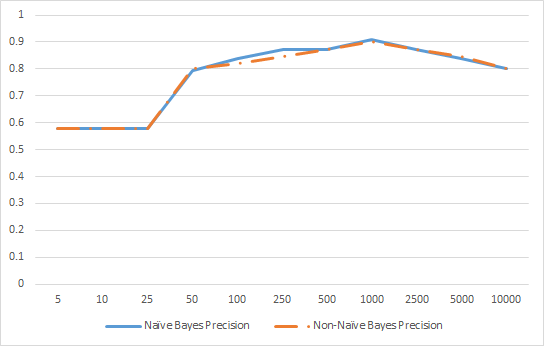
\includegraphics[width=120mm]{Precision.png}
	\caption{Precision}
	\label{PrecisionGraph}
\end{figure}

Overall precision of the classifier does not change noticeably. It drops slightly for $n$ between $100$ and $1000$, but for smaller and larger values it sees a comparable improvement.

\begin{figure}[ht!]
	\centering
	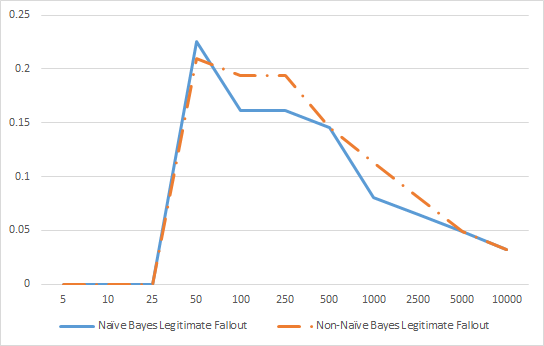
\includegraphics[width=120mm]{LegitimateFallout.png}
	\caption{Legitimate Fallout}
	\label{LegitimateFalloutGraph}
\end{figure}

Non-naive Bayesian classifier has slightly worse legitimate fallout score for $n$ between $100$ and $5000$, but is equal to or better than naive classifier's score for smaller and larger values. Performance of both classifiers converges as $n$ increases.

\begin{figure}[ht!]
	\centering
	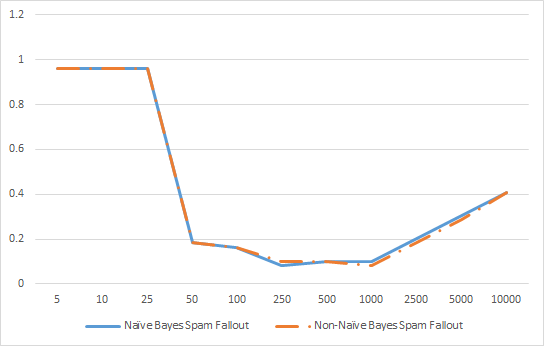
\includegraphics[width=120mm]{SpamFallout.png}
	\caption{Spam Fallout}
	\label{SpamFalloutGraph}
\end{figure}

In case of spam fallout the non-naive version performs better for most values and like in case of legitimate fallout it converges to naive classifier's fallout.

The average performance does not change to a significant amount, which means that the assumption of feature independence does not impact the classifier's performance enough to consider non-naive version of the classifier in practice. For the same configuration of loss function the naive classifier actually tends to perform better in terms of false negatives.

Another interesting point is that usage of all available features does not increase, but instead hurts the total precision of the naive classifier. This can be seen in Figure 5.1, where the precision reaches its maximum value at around $1000$ features ($~4,6\%$ of available words), where both classifiers show equal precision of $90,1\%$.

The maximum depth of search in the trie for the given test set was $35\%$, while the average stayed at just $0,025\%$. This explains the close results of both classifiers since only a small number of conditional probabilities have different values in non-naive classifier, therefore the overall probability $P(x | c)$ did change much from an approximation in naive approach. The average depth of trie search can potentially be improved by putting the features with close values $P(x_i = 1 | c)$ and $P(x_i = 0 | c)$ for both $c = L$ and $c = S$. However, the mutual information value for these features will be lowest, therefore there is not much use of having precise conditional probabilities for these features instead of features with higher mutual information.

In case of other classifiers, they have been tested on the same spam corpus in \cite{Tretyakov}. In case of all available $21700$ features the simple perceptron demonstrates the best precision of $98,5\%$, followed by SVM with precision of $98,1\%$. $k$ Nearest Neighbors and Naive Bayes perform worse with precision of $90,8\%$ and $87,4\%$ respectively. However, despite having the worst precision, naive Bayesian classifier has $0$ legitimate fallout, which makes it a great choice for spam filtering with minimal to no effort in tweaking the loss function. Also, note that its performance is not optimal for the large number of features, as it reaches precision of $90,1\%$ at $n = 1000$ on the same dataset.

\newpage


\chapter*{Conclusion}
\addcontentsline{toc}{chapter}{Conclusion}

The problem targeted in this thesis is statistical approaches to spam filtering in the most generic case, without domain specific properties. These constraints allowed to apply a number of different approaches under identical requirements, which both makes the solutions more universal and enables direct comparisons of different methods.

In particular we analyzed the simplest and most common method of spam detection - naive Bayesian classifier. While it guarantees to minimize the average classification risk, it does rely on an incorrect assumption of independence of features. A number of improvements that tackle this assumption were proposed, including partial optimizations that allow to balance guarantees and classification speed.

The results obtained in practice show no significant difference between the original classifier and the proposed modification which takes feature dependence into account. The primary reason behind this is that on average only a small fraction ($0,025\%$) of actual conditional probabilities of separate features were computed, while the others were approximated with their naive values. This can be interpreted as an effect of Bayesian classifier being optimal in the context of its training set, which means that formal probability for feature vectors which are not present in the training set is zero. Therefore, increased effect requires a significantly larger training set.

Therefore, in practice the benefit of non-naive versions of Bayesian classifier are negligible compared to additional requirements to the storage subsystem. Storing $O(nk)$ data structure that allows efficient calculations of chain probabilities is not always feasible in practice. In our case it limited the number of features that could be used for classification. However, modifications with limited depth of the search trie are also possible, allowing to achieve performance close to non-naive classifier with little overhead.

Finally, when compared to other approaches, the updated Bayesian classifier does produce similar or better results than k nearest neighbors, while usually being behind the perceptron and SVM. Still, it has a number of benefits over alternative methods. Firstly, it is the best default option in case of expensive false positives, which can be a critical requirement in spam filtering. Secondly, the quality of classification only improves with larger training sets, when for other classifiers it might cause problems with non-separable data. Finally, it reaches maximum performance with relatively small number of available features, allowing to use significantly larger training sets with the same speed and storage requirements.

\newpage


\addcontentsline{toc}{chapter}{References}

\begin{thebibliography}{30}

\bibitem{Tretyakov} K. Tretyakov 2004. Machine Learning Techniques in Spam Filtering. Institute of Computer Science, University of Tartu. Data Mining Problem-oriented Seminar, MTAT.03.177, May 2004, pp. 60-79.

\bibitem{Christina} V.Christina, S.Karpagavalli, G.Suganya 2010. Email Spam Filtering using Supervised Machine Learning Techniques. 2010, (IJCSE) International Journal on Computer Science and Engineering Vol. 02, No. 09, 2010, 3126-3129.

\bibitem{Kecman} V. Kecman 2001. Learning and Soft Computing. 2001, The MIT Press.

\bibitem{Zhang} H. Zhang 2004. The Optimality of Naive Bayes. Faculty of Computer Science, University of New Brunswick Fredericton.

\bibitem{Androutsopoulos} I. Androutsopoulos 2000. An Experimental Comparison of Naive Bayesian and Keyword-Based Anti-Spam Filtering with Personal E-mail Messages.

\bibitem{Sahami} M. Sahami, S. Dumais, D. Heckerman, and E. Horvitz 1998. A Bayesian approach to filtering junk email., AAAI Workshop on Learning for Text Categorization, July 1998, Madison, Wisconsin. AAAI Technical Report WS-98-05.

\bibitem{Haykin} S. Haykin 1998. Neural Networks: A Comprehensive Foundation. 1998, Prentice
Hall.

\bibitem{Cristianini} N. Cristianini, J. Shawe-Taylor 2003. An Introduction to Support Vector Machines and other kernel-based learning methods. 2003, Cambridge University Press. http://www.support-vector.net

\bibitem{Zaffalon} M. Zaffalon, M. Hutter 2002. Robust Feature Selection by Mutual Information Distributions. https://arxiv.org/ftp/arxiv/papers/1408/1408.1487.pdf

\end{thebibliography}


\end{document}